%\documentclass[../examplethesis.tex]{subfiles}
%\begin{document}
\chapter{DiVA administrator viewpoint}
\label{ch:adminViewpoint}

This chapter, written by Gerald Q. Maguire Jr.,  describes the implications of the thesis templates I have developed for use at KTH from the viewpoint of a DiVA administrator. Other documents provide the template which also contains information for authors and information about why the template is the way that it is. This document provides some information for DiVA administrators about the template and how it can be used with some programs to help make the degree process easier for students, faculty, and administrators while at the same time \textbf{greatly} reducing the work needed to report a thesis into DiVA.

An assumption for readers of this document is that you know KTH-speak, including the various acronyms that are used.

\textbf{This document is a work in progress.}

\section[Introduction to templates for DiVA administrators]{Introduction to templates for\\ DiVA administrators}

The assumption is that a student has written their thesis starting with either a DOCX document or \LaTeX\~project that have used the thesis templates; these are marked as ``DOCX using template'' and ``\LaTeX project using template'' (respectively), see \Cref{fig:forDiVAAdmins}. The key idea is to have these sources include  \first the information that is need for input into DiVA and \Second the information that can be used to produce and apply a cover to the resulting PDF file that will be uploaded into DiVA (either just for archiving or for also making the full-text available).

The ``DOCX using template'' and ``\LaTeX project using template'' are input to their respective programs as usual by the student to produce a PDF file (marked as ``PDF using template'') and possibly other files. This PDF file has one or more pages at the end of it that are in a section with a heading of ``For DIVA'' or this same string with four euro symbols (\ie `€') before and after the string with a space before and after the string. An example of the top of such a page is shown in \Cref{fig:topOfForDiva}.  At a minimum all of the data is now collected in one spot from which in the worst case one can cut-and-paste it into a single JSON file; however, some programs have been developed to mechanically extract this data, as will be described in \Cref{sec:gettingNecessaryData} - thus avoiding the need to cut-and-paste $\Rightarrow$ more fika time.

\tikzset{
    processBox/.style={rectangle, rounded corners, minimum width=3cm, minimum height=1cm,text centered, draw=black, fill=red!20},
    destinationBox/.style={rectangle, rounded corners, minimum width=3cm, minimum height=1cm,text centered, draw=black, fill=green!10},
    arrow/.style={thick,->,>=stealth}
}

\begin{figure}[!ht]
\resizebox{1.1\textwidth}{!}{%
\begin{tikzpicture}
[align=left,node distance=2cm]



\node (DOCXFile) [tape,tape bend top=none,draw,font=\sffamily] {DOCX using template};
\node (latexFile) [tape,tape bend top=none,draw,font=\sffamily, right=0.5cm of DOCXFile] {\LaTeX project using template};




\node (LaTeX) [processBox,  below=5cm of latexFile] {LaTeX compiler};
\node (latexjsonFile) [tape,tape bend top=none,draw,font=\sffamily, below of=LaTeX] {fordiva.json};



\node (extractDOCX) [processBox, below=8cm of DOCXFile] {extract\_custom\_DOCX\_properties};
\node (PDFfile) [tape,tape bend top=none,draw,font=\sffamily, left=5cm of LaTeX] {PDF using template};
\node (Word) [processBox,  above=3cm of PDFfile] {Word or similar};
\node (extractor) [processBox, below=6cm of PDFfile] {extract\_pseudo\_JSON-from\_PDF};

\node (cleanJSONfromLaTeX) [processBox, below=4cm of LaTeX] {cleanup\_pseudo\_JSON-from\_LaTeX};
\node (jsonFile) [tape,tape bend top=none,draw,font=\sffamily, below=4cm of cleanJSONfromLaTeX] {JSON file};

\node (assignTRITA) [processBox, below=3cm of jsonFile] {Assign TRITA number};
\node (jsonFileWithTRITA) [tape,tape bend top=none,draw,font=\sffamily, below of=assignTRITA] {JSON file with TRITA};
\node (jsontoMODS) [processBox, below of=jsonFileWithTRITA] {JSON\_to\_MODS};

\node (acronymsfile) [tape,tape bend top=none,draw,font=\sffamily, right=4.5cm of cleanJSONfromLaTeX] {acronyms.tex};

\node (TRITAlist) [destinationBox, right=1cm of assignTRITA] {TRITA list/database};

\node (modsFileWithTRITA) [tape,tape bend top=none,draw,font=\sffamily, below of=jsontoMODS] {MODS file with TRITA};
\node (makeApplyCover) [processBox, below of=modsFileWithTRITA] {Make and apply cover};
\node (divameta) [destinationBox, right=1cm of modsFileWithTRITA] {Import MODS file into DiVA};
\node (diva) [destinationBox, right=1cm of makeApplyCover] {Upload PDF into DiVA};


\draw [red, dashed]   (PDFfile) to[out=-120,in=180] (makeApplyCover);
\draw [red, dashed]   (Word) to[out=-90,in=90] (PDFfile);
\draw [red, dashed]   (LaTeX) to[out=-180,in=90] (PDFfile);
\draw [arrow] (DOCXFile) --  (extractDOCX.north);
\draw [arrow] (extractDOCX) --  (jsonFile.north west);
\draw [arrow] (latexFile.south) --  (LaTeX.north);
\draw [arrow] (LaTeX) --  (latexjsonFile.north);
\draw [arrow] (latexjsonFile) --  (cleanJSONfromLaTeX.north);
\draw [arrow] (cleanJSONfromLaTeX.south) --  (jsonFile.north);
\draw [red, dashed] (PDFfile) --  (extractor.north);
\draw [arrow] (DOCXFile) --  (Word.north);
\draw [arrow] (extractor.south) --  (jsonFile.west);
\draw [arrow] (jsonFile) --  (assignTRITA);
\draw [arrow] (jsontoMODS) --  (modsFileWithTRITA);
\draw [arrow] (modsFileWithTRITA) --  (divameta);
\draw [arrow] (assignTRITA) --  (jsonFileWithTRITA);
\draw [arrow] (jsonFileWithTRITA) --  (jsontoMODS);
\draw [arrow] (modsFileWithTRITA) --  (makeApplyCover);
\draw [arrow] (makeApplyCover) --  (diva);
\draw [arrow] (latexFile.south east) --  (acronymsfile.north);
\draw [arrow] (acronymsfile.south east) to[out=-45,in=0]  (jsontoMODS.east);
\draw [arrow] (TRITAlist) --  (assignTRITA.east);
\draw [arrow] (assignTRITA) --  (TRITAlist.west);

\end{tikzpicture}
}
\caption{Figure shows the flow of data relevant to DiVA administrators - the dashed red line shows the PDF, while the black lines show other types of data}
  \label{fig:forDiVAAdmins}
\end{figure}

\begin{figure}[!ht]
  \begin{center}
    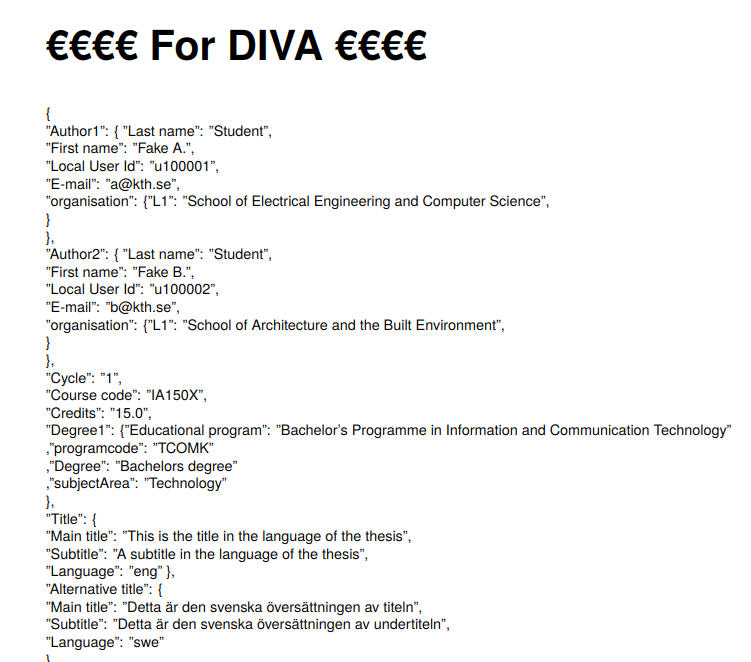
\includegraphics[width=0.99\textwidth]{README_notes/README-examiner-figures/for_diva_top_lines_Screenshot_20220403_164821.png}
  \end{center}
  \caption{Top of the page of data for DiVA}
  \label{fig:topOfForDiva}
\end{figure}
\FloatBarrier

\section{Getting the necessary data}
\label{sec:gettingNecessaryData}
The collected data shown in \Cref{fig:topOfForDiva} is roughly in a format called JavaScript Object Notation (JSON) and described in \Cref{sec:json}. There are several cases to consider for how to extract this information; then, given the information in JSON it is possible to generate a MODS file that can be imported into DiVA:
\begin{itemize}
    \item  \LaTeX~project - as described in \Cref{sec:extractingJSONLaTeX},
    \item DOCX file - as described in \Cref{sec:extractingJSONDOCX}, or
    \item PDF using template - as described in \Cref{sec:extractingJSONPDF}.
\end{itemize}


\subsection {JSON}
\label{sec:json}
JSON is a standard way of representing structured data as text. An example of this text is shown in \Cref{lst:forDIVAtop}. This format is useful as it is \first readily readable by both humans and computers and \Second is easy to edit, and \third is commonly supported by many programming languages. The basic element is of the form: \textquotedbl label\textquotedbl: value\ where label is a string and value can be another string or a structure (an element inside curly braces). String values are within double quote marks. A label of \textquotedbl First name\textquotedbl and the value \textquotedbl Fake A.\textquotedbl~is shown in line \ref{line:firstName} of the listing below. This is part of a structure that gives a value for \textquotedbl Author1\textquotedbl~and this value is a structure with a list of elements for \textquotedbl Last name\textquotedbl, \textquotedbl First name\textquotedbl, \textquotedbl Local User Id\textquotedbl~(\ie the kthid), \textquotedbl E-mail\textquotedbl, and \textquotedbl organisation \textquotedbl. The organisation in turn can have multiple levels where the first level L1 is the school, L2 is a department, and L3 is a division. In a discussion with DiVA administrators at KTH on 2021-04-29, the consensus was that the organizational affiliation of students should be the school of the thesis examiner, since 1\textsuperscript{st} and 2\textsuperscript{nd} cycle students are in \textbf{programs of study} and not schools, department, \etc.

\begin{lstlisting}[language=json, numbers=left,
    stepnumber=1, escapechar=|, caption={Text version of the top of the For DIVA output (reformatted to bring out the structure and improve readability - line numbers are added just in the listing)}, label=lst:forDIVAtop]
{
"Author1": { 
    "Last name": "Student",
    "First name": "Fake A.", |\label{line:firstName}|
    "Local User Id": "u100001",
    "E-mail": "a@kth.se",
    "organisation": {"L1": "School of Electrical Engineering and Computer Science",}
},
"Author2": {
    "Last name": "Student",
    "First name": "Fake B.",
    "Local User Id": "u100002",
    "E-mail": "b@kth.se",
    "organisation": {"L1": "School of Architecture and the Built Environment",}
},
"Cycle": "1",
"Course code": "IA150X",
"Credits": "15.0",
"Degree1": {
    "Educational program": "Bachelor's Programme in Information and Communication Technology",
    "Programcode": "TCOMK",
    "Degree": "Bachelors degree", |\label{line:degree}|
    "subjectArea": "Technology"   |\label{line:subjectarea}|
},
"Title": {
    "Main title": "This is the title in the language of the thesis",
    "Subtitle": "A subtitle in the language of the thesis",
    "Language": "eng" },
"Alternative title": {
    "Main title": "Detta är den svenska översättningen av titeln",
    "Subtitle": "Detta är den svenska översättningen av undertiteln",
    "Language": "swe"
},
\end{lstlisting}

\subsection{Case of \LaTeX~project}
\label{sec:extractingJSONLaTeX}

In the case of an \LaTeX~project, when compiling the \LaTeX~as a side-effect a \texttt{fordiva.json} file is generated, if you save this file locally then you can clean it up and make a MODS file with the following commands:
\Needspace*{4\baselineskip}
\begin{lstlisting}[basicstyle=\footnotesize, language={bash}, caption={Cleanup pseudo JSON produced by the \LaTeX~compiler and then make a MODS file},label=lst:AdmincleanPseudoJSONandConvertToMODS]
./cleanup_pseudo_JSON-from_LaTeX.py --json fordiva.json --acronyms acronyms.tex
./JSON_to_MODS.py --json fordiva-cleaned.json
\end{lstlisting}

Now all you have to do is rename the XML file (\texttt{modsXML.xml}) that was produced to \texttt{xxx.mods} and you are all set to upload the MODS file into DiVA!

To find the \texttt{fordiva.json} file in the \LaTeX project in Overleaf, look for the “Other logs and files” button shown at the bottom of the log output window. After clicking this button you will see a list of log and other files and can now download it.

Note that if the student has used the glossaries package to use acronyms in the abstract(s) they also need to provide an \texttt{acronyms.tex} file.

\generalExpl{Should the student submit the \texttt{fordiva.json} and \texttt{acronyms.tex} file via Canvas (along with their PDF file)?}

\subsection{Case of DOCX file}
\label{sec:extractingJSONDOCX}
In the case of a DOCX file using the template\footnote{The DOCX template (\eg Template-thesis-English-2022-with-for-DiVA.docx is available from available from \url{https://github.com/gqmaguirejr/E-learning} ) while information about using the DOCX template is in the document ``Proposal for a standard thesis template: DOCX version(s)'' available from the same GitHub.}, the JSON data can be extracted directly from the DOCX file and a MODS file created as shown in \Cref{lst:extractDOCX}.
\Needspace*{4\baselineskip}
\begin{lstlisting}[basicstyle=\footnotesize, language={bash}, caption={Extract field values from the DOCX file and then make a MODS file},label=lst:extractDOCX]
./extract_customDocProperties.py filename.docx --json output.json
./JSON_to_MODS.py --json output.json
\end{lstlisting}
If the –-json option is not included in the arguments to\linebreak[4] \texttt{extract\_customDocProperties.py}, the output file is by default “output.json”.

Note that the program can be given an argument of either \texttt{\hbox{–-English}} or \texttt{\hbox{–-Swedish}} to explicitly set the language for the body text. Otherwise, the choice is made based upon the default language (w:lang) specified in the word/settings.xml file.

\warningExpl{Perhaps a custom property for the language of the document should be added.}

The number of pages of the preface and body of the document is taken from the result of the page references to the two bookmarks as generated in the “For DIVA” data. One cannot derive this data directly but only by extracting the data from the word/document.xml file (\textit{after} the word processing package has generated the textual representation for these markers – since their values depends upon the layout and pagination of the document).

A major limitation is that this program only supports extracting English and Swedish abstracts (and keywords); hence abstracts in other languages are \textbf{not} extracted. Additionally, the support for HTML markup in the abstracts is limited to paragraphs. 


\generalExpl{Should the student submit the \texttt{output.json} file via Canvas (along with their PDF file)?}

\subsection{Case of PDF using template file}
\label{sec:extractingJSONPDF}
If all you have is a ``PDF using template file'' then one can extract the information using the program \texttt{extract\_pseudo\_JSON-from\_PDF.py}.  Given a ``PDF using template'' file (and if a \LaTeX~project has been used the acronyms.tex file):
\begin{enumerate}
    \item Save the PDF file of the thesis, for example: \texttt{oscar.pdf}
    \item Extract the “For DIVA” information as JSON, as shown in \Cref{lst:AdminextractPseudoJSONFromPDFforOscarFileToJSON}
    
    If acronyms are used in the abstracts, you can add the “--acronyms acronyms.tex” argument to the extract command line and the program will process the acronyms from the acronyms.tex file (this means that you will also need this file). The output of the program is a JSON file (oscar.json) that can subsequently be used to make an announcement.
\end{enumerate}
\Needspace*{7\baselineskip}
\begin{lstlisting}[basicstyle=\footnotesize, language={bash}, caption={Commands to extract pseudo JSON from the PDF file for Oscar}, label=lst:AdminextractPseudoJSONFromPDFforOscarFileToJSON]    
./extract_pseudo_JSON-from\_PDF.py --pdf oscar.pdf --json oscar.json
./JSON_to_MODS.py --json oscar.json
\end{lstlisting}

\generalExpl{Should the student submit the \texttt{xxxx.json} file and possibly the acronyms.text file via Canvas (along with their PDF file)?}

\subsection{TRITA}
Unless the Office of Student Affairs is going to assign TRITA numbers before the thesis has a cover made, then I think that the Office of Student Affairs has to assign the TRITA number and then \textbf{make and apply the cover}. The current method of making and applying covers before the PDF is submitted to the Office of Student Affairs is foolish and unnecessary. It is easy to specify the TRITA string as an argument when making the MODS file, as shown in \Cref{lst:specifyTRITA}. 
\begin{lstlisting}[basicstyle=\footnotesize, language={bash}, caption={Command to make a MODS file with a specified TRITA string}, label=lst:specifyTRITA]
./JSON_to_MODS.py --json fordiva.json --trita "TRITA-EECS-EX-2021:219"
\end{lstlisting}

This requires that the student provide the information about the degree that they will apply for and the subject area \textbf{within} their document so that it ends up in the JSON file. This was done in lines  \ref{line:degree} and \ref{line:subjectarea} in \Cref{lst:forDIVAtop}.

\subsection{Covers}
A DOCX cover can be made for a thesis using the \texttt{JSON\_to\_DOCX\_cover.py} command shown in \Cref{lst:JSONtoDOCXcover}. This command supports the many different types of exams. It also can take many optional parameters that will over ride the contents of the JSON file (by default the JSON file name is assumed to be \texttt{calendar\_event.json}) as shown in \Cref{lst:JSONtoDOCXcover2}. If the \texttt{\hbox{-\,-language sv}} command is used or the language of the main title is Swedish (indicate in the JSON file as `swe'') the program eliminates the English KTH logotype and changes the course name appropriately. The field of technology or main subject have to be in the selected language, shown in \Cref{lst:JSONtoDOCXcover2}. Note that you can optionally specify the TRITA string on the command line with an option of the form:
\texttt{\hbox{-\,-TRITA  "TRITA-EECS-EX-2022:99999"}}.

\begin{lstlisting}[escapechar=|, basicstyle=\footnotesize, language={bash}, caption={Command to make a cover DOCX file with a specified TRITA string}, label=lst:JSONtoDOCXcover]
./JSON_to_DOCX_cover.py --file  Omslag_Exjobb_Eng_en-20220325.docx |\textbackslash \\| --exam kandidatexamen  --trita "TRITA-EECS-EX-2021:219"
\end{lstlisting}

\begin{lstlisting}[escapechar=|, basicstyle=\footnotesize, language={bash}, caption={Command to make a cover DOCX file with the specified values}, label=lst:JSONtoDOCXcover2]
./JSON_to_DOCX_cover.py --file Omslag_Exjobb_Eng_en-20220325.docx|\textbackslash \\| --cycle 2 --credits 30.0 --area "bioteknik" --area2 "kemiteknik"|\textbackslash \\| --exam both --trita "TRITA-CBH-EX-2021:00"|\textbackslash \\| --language sv  --json calendar-sv.json
\end{lstlisting}

\textbf{NB}: The program is explicitly designed to work with the English version of the template from 2022-03-25, hence the specification of the template used in the two examples above.

\warningExpl{TODO: Make a program to make and apply the correct cover to the PDF file. Otherwise, one can use the specific templates shown at \url{https://canvas.kth.se/courses/11/pages/templates-for-1st-and-2nd-cycle-theses-some-templates}.}

\textbf{NB}: The current \LaTeX~template makes the front and back covers and uses a TRITA string specified in the \LaTeX~project files. The command shown in \Cref{lst:specifyTRITA} overrides this value when making the MODS file, but the existing TRITA string on the back cover has to be manually edited.

\warningExpl{Perhaps a solution is to integrate the \textbf{front} cover into both the \LaTeX and the DOCX templates and have the Office of Student Affairs apply only the back cover - as this is where the TRITA number appears.}

\textbf{NB}: The ``For DIVA'' pages need to be removed from the PDF file before uploading the PDF file into DiVA.

\section[Inserting information into LADOK]{Inserting information into LADOK}
\label{sec:JSONtoLADOKDiVAAdmis}
As part of the effort to be able to minimize the effort of cutting and pasting. I have made a program JSON\_to\_ladok.py that takes the extracted JSON information and uses the information about the author(s) and the title and alternative title to try to insert this information into LADOK for the module (\ie ``moment'' in Swedish) that requires a project title, \ie, 'KravPaProjekttitel' is True. \Cref{lst:usingExtractedJSONtoProduceLADOKentry1} shows an example of using this program to try to put the title and alternative title into LADOK. Basically the program logic should work, but I do \textbf{not} have the required permission to make entries of this sort of data for a degree project (\ie Rapporteringsrättighet saknas).

Note that this program uses the \texttt{ladok3} python library but extends it with some features that are not (yet) in the library. \textbf{It should be regarded as very much a work in progress.} However, it illustrates what could be done using the information in the JSON file.
\begin{lstlisting}[language={bash},
    breaklines=true,
    breakatwhitespace=true,          % sets if automatic breaks should only happen at whitespace
    breakindent=0em,
    caption={Using the extracted JSON to produce a LADOK entry for a student in the DA231X degree project course}, label=lst:usingExtractedJSONtoProduceLADOKentry1]
./JSON_to_ladok.py --json xxx.json 
...
author={'Last name': 'xxx', 'First name': 'yyy', 'Local User Id': 'u1xxxx', 'E-mail': 'oxxx@kth.se', 'organisation': {'L1': 'School of Electrical Engineering and Computer Science '}}
Canvas user_id=dddd
integration_id=gggggg-gggg-gggg-gggg-ggggggg
ladoK_course_info={'id': '6683207e-5a5d-11eb-9b32-eeb44fb14647', 'round_id': '8e15ae14-1d86-11ea-a622-3565135944de', 'education_id': '374ea085-73d8-11e8-afa7-8e408e694e54', 'instance_id': '8eee8da9-dd0a-11e8-bb7a-19f8cd1a470e', 'swe_name': 'Examensarbete i datalogi och datateknik, avancerad nivå', 'eng_name': 'Degree Project in Computer Science and Engineering, Second Cycle'}
moment code=PRO1, requires title=False
moment code=PRO2, requires title=False
moment code=PRO3, requires title=True
trying to store a passing grade for moment=PRO3
Traceback (most recent call last):
  File "./JSON_to_ladok.py", line 533, in <module>
    sys.exit(main(sys.argv[1:]))
  File "./JSON_to_ ladok.py", line 519, in main
    status=save_result_degree_project3(ladok, integration_id, course_code, mom['Utbildningskod'], '2021-07-14', 'P', "PF", main_title, alternative_main_title)
  File "./JSON_to_ ladok.py", line 374, in save_result_degree_project3
    raise Exception("Couldn't register " + course_moment + "=" + grade_raw + " " + result_date_raw + ": " + r.json()["Meddelande"])
Exception: Couldn't register PRO3=P 2021-07-14: Hinder mot skapa resultat påträffat: Rapporteringsrättighet saknas
\end{lstlisting}

\warningExpl{There is currently a transfer to LADOK project within the group of developers at the IT unit who are working on E-learning - they have been working on an API for entering the title(s) and other information (just as they are making it possible to use a program to enter grades and dates for other courses).}


\section{The examiners can also use the JSON file}

\Cref{fig:overallDataflow} shows the overall data flow starting with either a DOCX document or \LaTeX\~project that has used the thesis templates. Not only is the JSON data useful with respect to DiVA, but it can also be used for other purposes. For example, as shown in \Cref{fig:overallDataflow}, an examiner can use it for announcing the student's oral presentation via the Canvas course room and calendar and potentially in the KTH Cortina Calendar.

However, as calendar entries were not relevant to DiVA administrators, this figure was simplified in \Cref{fig:forDiVAAdmins}.

\begin{figure}[!ht]
\resizebox{1\textwidth}{!}{%
\begin{tikzpicture}
[align=left,node distance=2cm]



\node (DOCXFile) [tape,tape bend top=none,draw,font=\sffamily] {DOCX using template};
\node (latexFile) [tape,tape bend top=none,draw,font=\sffamily, right=0.5cm of DOCXFile] {\LaTeX project using template};




\node (LaTeX) [processBox,  below=5cm of latexFile] {LaTeX compiler};
%\node (acronymsfile) [tape,tape bend top=none,draw,font=\sffamily, right=2cm of latexFile] {acronyms.tex};
\node (latexjsonFile) [tape,tape bend top=none,draw,font=\sffamily, below of=LaTeX] {fordiva.json};



\node (extractDOCX) [processBox, below=8cm of DOCXFile] {extract\_custom\_DOCX\_properties};
\node (PDFfile) [tape,tape bend top=none,draw,font=\sffamily, left=5cm of LaTeX] {PDF using template};
\node (Word) [processBox,  above=3cm of PDFfile] {Word or similar};
\node (extractor) [processBox, below=6cm of PDFfile] {extract\_pseudo\_JSON-from\_PDF};

\node (cleanJSONfromLaTeX) [processBox, below=4cm of LaTeX] {cleanup\_pseudo\_JSON-from\_LaTeX};
\node (jsonFile) [tape,tape bend top=none,draw,font=\sffamily, below=4cm of cleanJSONfromLaTeX] {JSON file};

\node (start) [processBox, right=0.5cm of jsonFile] {JSON\_to\_calendar};

\node (assignTRITA) [processBox, below=3cm of jsonFile] {Assign TRITA number};
\node (jsonFileWithTRITA) [tape,tape bend top=none,draw,font=\sffamily, below of=assignTRITA] {JSON file with TRITA};
\node (jsontoMODS) [processBox, below of=jsonFileWithTRITA] {JSON\_to\_MODS};
%\node (modsFile) [tape,tape bend top=none,draw,font=\sffamily, below of=jsontoMODS] {MODS file};

\node (calendarEvent) [destinationBox, right=1cm of start] {Canvas calendar event};
\node (announcement) [destinationBox,  above of =calendarEvent] {Canvas announcement};
\node (acronymsfile) [tape,tape bend top=none,draw,font=\sffamily, right=4.5cm of cleanJSONfromLaTeX] {acronyms.tex};
\node (cortinaCalendarEvent) [destinationBox,  right=0.5cm of start, below of=calendarEvent] {KTH Cortina calendar event};
\node (TRITAlist) [destinationBox, right=1cm of assignTRITA] {TRITA list/database};

\node (modsFileWithTRITA) [tape,tape bend top=none,draw,font=\sffamily, below of=jsontoMODS] {MODS file with TRITA};
\node (makeApplyCover) [processBox, below of=modsFileWithTRITA] {Make and apply cover};
\node (divameta) [destinationBox, right=1cm of modsFileWithTRITA] {Import MODS file into DiVA};
\node (diva) [destinationBox, right=1cm of makeApplyCover] {Upload PDF into DiVA};


\draw [red, dashed]   (PDFfile) to[out=-120,in=180] (makeApplyCover);
\draw [red, dashed]   (Word) to[out=-90,in=90] (PDFfile);
\draw [red, dashed]   (LaTeX) to[out=-180,in=90] (PDFfile);
\draw [arrow] (DOCXFile) --  (extractDOCX.north);
\draw [arrow] (extractDOCX) --  (jsonFile.north west);
\draw [arrow] (latexFile.south) --  (LaTeX.north);
\draw [arrow] (LaTeX) --  (latexjsonFile.north);
\draw [arrow] (latexjsonFile) --  (cleanJSONfromLaTeX.north);
\draw [arrow] (cleanJSONfromLaTeX.south) --  (jsonFile.north);
\draw [red, dashed] (PDFfile) --  (extractor.north);
\draw [arrow] (DOCXFile) --  (Word.north);
\draw [arrow] (extractor.south) --  (jsonFile.west);
\draw [arrow] (jsonFile) --  (assignTRITA);
\draw [arrow] (jsonFile) --  (start.west);
\draw [arrow] (start.east) --  (announcement.west);
\draw [arrow] (start.east) -- (calendarEvent);
\draw [arrow] (start.east) -- (cortinaCalendarEvent.west);
%\draw [arrow] (jsonFile) --  (jsontoMODS.north west);
%\draw [arrow] (jsontoMODS) --  (modsFile);
%\draw [arrow] (jsontoMODS) --  (modsFile);
\draw [arrow] (jsontoMODS) --  (modsFileWithTRITA);
%\draw [arrow] (modsFile) --  (assignTRITA);
\draw [arrow] (modsFileWithTRITA) --  (divameta);
\draw [arrow] (assignTRITA) --  (jsonFileWithTRITA);
\draw [arrow] (jsonFileWithTRITA) --  (jsontoMODS);
\draw [arrow] (modsFileWithTRITA) --  (makeApplyCover);
\draw [arrow] (makeApplyCover) --  (diva);
%\draw [arrow] (assignTRITA) --  (modsFileWithTRITA);
\draw [arrow] (latexFile.south east) --  (acronymsfile.north);
\draw [arrow] (acronymsfile.south east) to[out=-45,in=0]  (jsontoMODS.east);
\draw [arrow] (TRITAlist) --  (assignTRITA.east);
\draw [arrow] (assignTRITA) --  (TRITAlist.west);

\end{tikzpicture}
}
\caption[Overall data flow]{Overall data flow from a DOCX document and a \LaTeX\~project using the templates. The figure shows the flow of data - the dashed red line shows the PDF, while the black lines show other types of data}
  \label{fig:overallDataflow}
\end{figure}
\FloatBarrier
\section{Open questions}
Some of the open questions are:
\begin{itemize}
    \item What should the student submit (via the examiner or via Canvas?)?
    \item What should the Office of Student Affairs do?
\end{itemize}

\section{Final notes}
\textbf{Best of success in using the programs!} If there are questions, contact me at  \href{mailto:maguire@kth.se}{maguire@kth.se}
.

%\end{document}
